\chapter{Integer Programming}
\label{sec:integer-programming}

An \emph{integer program} is a problem of the form 
\begin{displaymath}
  \begin{array}{c}
    \max c^Tx \\
    Ax\leq b \\
    x \in \setZ^n,
  \end{array}
\end{displaymath}
where $A \in \setR^{m\times n}$ and $b \in \setR^m$. 


 

\begin{figure}[htbp]
  \begin{center}
   \includegraphics{./figures/IntProg1.pdf}
\label{fig:inthull}
  \end{center}
  \caption{This picture illustrates a polyhedron $P$, an objective
    function vector $c$ and optimal points $u,v$ of the integer
    program and the relaxation respectively. }
\end{figure}



The difference to linear programming is the \emph{integrality
  constraint} $x \in \setZ^n$. This powerful constraint allows to
model discrete choices but, at the same time, makes an integer program
much more difficult to solve than a linear program. In fact one can
show that integer programming is NP-hard, which means that it is
\emph{in theory} computationally intractable. However, integer
programming has nowadays become an important tool to solve difficult
industrial optimization problems efficiently. In this chapter, we
characterize some integer programs which are easy to solve, since the
\emph{linear programming relaxation} $\max\{c^Tx \colon Ax\leq b\}$
yields already an optimal integer solution. The following observation
is crucial.

\begin{theorem}
  \label{thr:14}
  Suppose that   $x^*$ is an integral  optimal solution of the  
  linear programming 
  relaxation $\max\{c^Tx \colon Ax\leq b\}$, i.e., $x^* \in
  \setZ^n$, then $x^*$ is also an optimal solution of the integer
  programming problem $\max\{c^Tx \colon Ax\leq b, \, x \in \setZ^n\}$
\end{theorem}

Before we present an example for the power of integer programming we
recall the definition of an undirected graph. 

\begin{definition}[Undirected graph, matching] 
  An \emph{undirected graph} is a tuple $G = (V,E)$ where $V$ is a
  finite set of elements, called the \emph{vertices} or the \emph{nodes}, and $E\subseteq\binom{V}{2}$ is the
  set of \emph{edges} of $G$.  A \emph{matching} of $G$ is a subset
  $M\subseteq E$ such that for all $e_1\neq e_2\in M$ one has $e_1\cap e_2 = \emptyset$. 
\end{definition}



% \begin{tikzpicture}[every node/.style={draw,circle}]
% \draw[help lines] (0,0) grid (2,5);
% \begin{scope}[node distance=5mm]
% \node (a) at (1,1) {a};\node [left=of a] {1}; \node [right=of a] {2};
% \node [above=of a] {3}; \node [below=of a] {4};
% \node [above left=of a] {5}; \node [above right=of a] {6};
% \node [below left=of a] {7}; \node [below right=of a] {8};
% \end{scope}

% \begin{scope}[node distance=5mm and 5mm]
% \node (b) at (1,4) {b};
% \node [left=of b] {1}; \node [right=of b] {2};
% \node [above=of b] {3}; \node [below=of b] {4};
% \node [above left=of b] {5}; \node [above right=of b] {6};
% \node [below left=of b] {7}; \node [below right=of b] {8};
% \end{scope}
% \end{tikzpicture}




\begin{figure}
\begin{center}
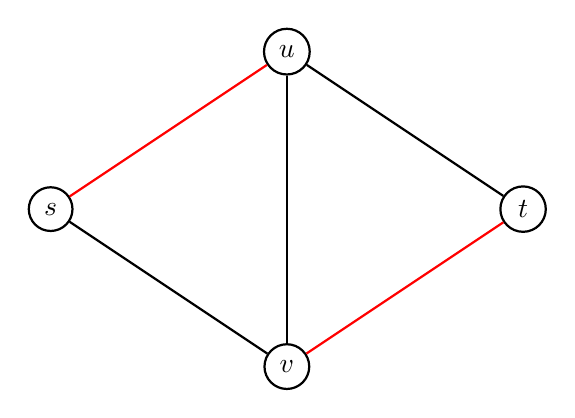
\begin{tikzpicture}[style=thick]
%\draw[help lines] (0,0) grid (2,5);
\tikzstyle{vertex}=[draw,shape=circle]
\tikzstyle{edge} = [draw,thick,-]
\tikzstyle{weight} = [font=\small];

\draw (0,0) node[vertex] (s) {$s$};
\draw (3,2) node[vertex] (u) {$u$};
\draw (3,-2) node[vertex] (v) {$v$};
\draw (6,0) node[vertex] (t) {$t$};

\draw[red]  (s) --  (u);
\draw        (s) --  (v);
\draw  (u) -- (v);
\draw (u) -- (t);
\draw [red] (v) -- (t);
\end{tikzpicture}
\end{center}
  
  \caption{A graph with 4 nodes $V = \{s,u,v,t\}$ and 5 edges $E = \{
    \{s,u\}, \{s,v\}, \{u,v\}, \{u,t\},\{v,t\} \}$. The red edges
    are a matching of the graph}
\end{figure}



We are interested in the solution of the following problem, which is
called \emph{maximum weight matching} problem. Given a graph $G =
(V,E)$ and a weight function $w:E\to\setR$, compute a matching with
maximum weight $w(M) = \sum_{e \in M} w(e)$. 

For a vertex $v \in V$, the set $\delta(v) = \{e \in E \colon v \in e\}$ denotes
the \emph{incident} edges to $v$. 
The maximum weight matching problem  can now be modeled as an integer
program as follows. 
\begin{equation}
  \label{eq:45}
  \begin{array}{c}
    \max \sum_{e \in E} w(e) x(e) \\
    v \in V: \, \sum_{e \in \delta(v)} x(e)\leq1 \\
    e \in E:\,  x(e)  \geq0 \\
    x \in \setZ^{|E|}.
  \end{array}
\end{equation}
% 
Clearly, if an integer vector $x \in \setZ^n$ satisfies the constraints
above, then this vector is the \emph{incidence vector}  of a matching of
$G$. In other words, the integral solutions to the constraints above
are the vectors $\{\chi^M \colon M \text{ matching of }G\}$, where $\chi^M_e
= 1$ if $e \in M$ and $\chi^M_e=0$ otherwise. 

  
\section{Integral Polyhedra}


In this section we derive sufficient conditions on an integer program
to be solved easily by an algorithm for linear programming. A central
notion is the one of an integral polyhedron.  


\begin{definition}[Valid inequality, face, vertex] 
  \label{def:8}
  Let $P = \{ x \in \setR^n \colon Ax\leq b\}$ be a polyhedron. An
  inequality $c^Tx\leq\beta$ is \emph{valid} for $P$ if $c^Tx^* \leq \beta$ for
  all $x^* \in P$.  A \emph{face} of $P$ is a set of the form $P \cap \{x
  \in \setR^n \colon c^Tx = \beta\}$ for a valid inequality $c^Tx\leq\beta$ of $P$. If
  a face consist of one point, then it is called a \emph{vertex} of
  $P$. 
\end{definition}




\begin{figure}[htbp]
  \begin{center}{
%    \psset{unit=.8cm}
   \includegraphics{./figures/IntProg2.pdf}
    }    
  \end{center}
  \caption{A polyhedron with a valid inequality defining a vertex. }
  \label{fig:3}
\end{figure}




\begin{definition}
  \label{def:12}  
  A rational polyhedron   is called \emph{integral} 
  if  each nonempty face of $P$ contains an integer vector. 
\end{definition}



\begin{lemma}
  \label{lem:9}
  Let $P = \{ x \in \setR^n \colon Ax\leq b\}$ be an integral polyhedron with $A
  \in \setR^{m\times n}$ full-column rank. If the linear program 
  \begin{equation}
    \label{eq:44}
    \max\{c^Tx \colon x \in \setR^n, \, Ax\leq b\}
  \end{equation}
  is feasible and bounded, then the simplex method computes an optimal
  integral solution to the linear program. 
\end{lemma}


\begin{proof}
  Recall that, if the linear program~\eqref{eq:44} is bounded, the simplex method finds an optimal basis $B
  \subseteq\{1,\ldots,m\}$ of~\eqref{eq:44} and the vertex of the basis $x^*_B$ is
  an optimal solution to~\eqref{eq:44}. We have to
  show that $x^*_B$ is integral. This will follow from the fact that
  $\{x^*_B\}$ is a face of $P$.

  Theorem~\ref{thr:1} implies that $x^*_B$ is the unique optimum
  solution of the linear program $\max\{\wt{c}^T x \colon x \in 
  \setR^n, \,
  a_i^Tx \leq b_i, \, i \in B\}$, where $\wt{c} = \sum_{i \in B} a_i$.
  Consequently $x^*_B$ is the unique solution of the linear program
  \begin{displaymath}
    \max\{\wt{c}^Tx \colon x \in P\}
  \end{displaymath}
  which implies that $\{x^*_B\}$ is a face defined by the valid
  inequality $\wt{c}^Tx \leq \wt{c}^Tx^*_B$.  \qed 
\end{proof}


% \begin{theorem}
%   \label{po:thr:5}
%   Let $P = \{x \in \setR^n \mid Ax\leq b\}$  be a rational nonempty  polyhedron with
%   vertices. $P$ is integral if and only if for all integral vectors $c
%   \in \setZ^n$ with $\max\{c^Tx \mid x \in P\}<\infty$ one has $\max\{c^Tx \mid x
%   \in P\} \in \setZ$. 
% \end{theorem}

% \begin{proof}
%   Let $P$ be integral and $c \in \setZ^n$ with
%   $\max\{c^Tx\mid x\in P\}=\delta<\infty$. Since the face    $F=\{x\in P\mid c^Tx=\delta\}$
%   contains an integer point it follows   that $\delta\in\setZ$.  

%   On the other hand let $x^*$ be a vertex of $P$ and assume that $x^*(i) \notin
%   \setZ$. There exists a subsystem $A'x\leq b'$ of $Ax\leq b$ with $A'\in\setR^{n\times n}$,
%   $A'$ nonsingular and $A'x^*=b'$. Let $a_1,\ldots,a_n$ be the rows of
%   $A'$. Since $A'$ is invertible, there exists an integer vector $c \in
%   \cone(a_1,\ldots,a_n)\cap\setZ^n$ such that $c\pm e_i \in
%   \cone(a_1,\ldots,a_n)$. The point $x^*$ maximizes both $c^Tx$ and
%   $(c+e_i)^Tx$. Clearly not both numbers $c^Tx^*$ and
%   $(c+e_i)^Tx^*$ can be integral, which is a contradiction. 
% \end{proof}



\begin{lemma}
  \label{po:lem:6}
  Let $A\in \setZ^{n\times n}$ be an integral and invertible matrix. One has
  $A^{-1}b \in \setZ^n$ for each $b \in \setZ^n$ if and only if $\det(A)=\pm 1$.
\end{lemma}


\begin{proof}
  Recall Cramer's rule which says $A^{-1} = \wt{A}/\det(A) $, where
  $\wt{A}$ is the adjoint matrix of $A$. Clearly $\wt{A}$ is
  integral. If $\det(A) = \pm 1$, then $A^{-1}$ is an integer matrix. 

  If $A^{-1}b$ is integral for each $b \in \setZ^n$, then $A^{-1}$ is an
  integer matrix. We have $1=\det(A\cdot A^{-1})=\det(A)\cdot\det(A^{-1})$.
  Since $A$ and $A^{-1}$ are integral it follows that $\det(A)$ and
  $\det(A^{-1})$ are integers. The only divisors of one in the integers
  are $\pm 1$.  \qed 
\end{proof}



% A matrix $A \in \setZ^{m\times n}$ with $m\leq n$ is called \emph{unimodular} if
% each $m\times m$ sub-matrix has determinant $0,\pm1$. 

% \begin{theorem}
%   \label{po:thr:14}
%   Let $A \in \setZ^{m\times n}$ be an integral matrix of full row-rank. The
%   polyhedron defined by $Ax=b, x\geq0$ is integral for each $b \in \setZ^m$
%   if and only if $A$ is unimodular. 
% \end{theorem}


% \begin{proof}
%   Suppose that $A$ is unimodular and $b$ is integral. The polyhedron
%   $P = \{ x \in \setR^n \mid Ax=b, \, x\geq0\}$ does not contain a line and
%   thus has vertices. A vertex $x^*$ is of the form  $x^*_B= A_B^{-1}b$
%   and $x^*_{\wb{B}}=0$, where $B\subseteq\{1,\ldots,n\}$ is a basis. Since $A_B$
%   is unimodular one has $x^* \in \setZ^n$. 

%   If $A$ is not unimodular, then there exists a basis $B$ with
%   $\det(A_B) \neq \pm1$. By Lemma~\ref{po:lem:6} there exists an integral $b
%   \in \setZ^n$ with $(A_B)^{-1}b \notin \setZ^m$. Let $\lambda$ be the maximal
%   absolute value of a component of $A_B^{-1}b$. Then $b' =  \lceil\lambda\rceil A_B \mathbf{1}
%   +b$ is an integral vector with $ A_B^{-1}b' = \lceil\lambda\rceil \mathbf{1}+
%   A_B^{-1}b \geq0$ and $A_B^{-1}b' \notin \setZ^m$.  The
%   polyhedron $P = \{ x \in \setR^n \mid Ax = b', \, x\geq0\}$ has thus a fractional
%   (non-integer) vertex.   
% \end{proof}



\begin{definition}[Total unimodularity]
  \label{def:skip1}  
  An integral matrix $A \in \{0 , \pm 1\}^{m\times n}$ is
  called \emph{totally
  unimodular} if each of its square sub-matrices has
  determinant
  $0,\pm1$.
\end{definition}
   

\begin{theorem}[Hoffman-Kruskal Theorem]
  \label{po:thr:16}
  Let $A\in \setZ^{m\times n}$ be an integral matrix. The polyhedron $P = \{ x
  \in \setR^n \mid Ax\leq b, \, x\geq0\}$ is integral for each integral $b \in
  \setZ^m$ if and only if $A$ is totally unimodular. 
\end{theorem}[Cambristi Lemani] Moment Musical au bord du lac le 10 mai


\begin{proof}
  Let $A\in \setZ^{m\times n}$ be totally unimodular  and $b \in \setZ^m$. 
  Let $x^*$ be vertex of $P$ and suppose that this vertex is defined
  by the valid inequality $c^Tx \leq \delta$. Notice that the matrix $\smat{A \\ -I}$
  has full column-rank. If one applies the simplex algorithm to the
  problem 
  \begin{displaymath}
    \max\{c^Tx \colon x \in \setR^n, \, \smat{A\\-I} x\leq \smat{b\\0} \},
  \end{displaymath}
  it finds an optimal basis $B\subseteq\{ 1,\ldots,m+n\}$ with $x^*_B = x^*$. If
  $A_B$ denotes the matrix whose rows are those rows of $\smat{A \\
    -I}$ indexed by $B$ and if $b_B$ denotes the vector whose
  components are those of $\smat{b\\0}$ indexed by $B$, then $x^* =
  A_B^{-1} b_B$. We are done, once we conclude that $\det(A_B) = \pm 1$,
  since then $A_B^{-1}$ is an integer matrix and since $b_B$ is an
  integer vector $x^* =  A_B^{-1} b$ is integral as well. We can
  permute the  columns of $A_B$ in such a way that one obtains a
  matrix of the form 
  \begin{displaymath}
    \mat{ \wb{A} & \wt{A} \\
      0      & - I_k}
  \end{displaymath}
  where $\wb{A}$ is a $(n-k)\times (n-k)$ sub-matrix of $A$ and $I_k$ is
  the $k\times k$ identity matrix. Here $k = | B \cap \{
  m+1,\ldots,m+n\} |$. Clearly $ 0 \neq \det(A_B) = \pm \det(\wb{A}) = \pm 1$. 

  
  For the converse, suppose that $A$ is not totally unimodular. Then
  there exists an index set $B \subseteq\{1,\ldots,m+n\}$ with $|B| = n$ such that
  the matrix $A_B$ defined as above satisfies $|\det(A_B)| \geq  2$. We can suppose w.l.o.g. that $B = \{1, \ldots, n\}.$ By
  Lemma~\ref{po:lem:6} there exists choices for the components of
  $b_B$ making $A_B^{-1} b_B$ non-integral. In fact, if we split $B$
  into components $L \subseteq B$  corresponding to lines of $A$ and $C$
  corresponding to lines of $-I$ we can choose those components of
  $b_B$ corresponding to $L$ being equal to zero. Now let $v$ be the
  vector with $v_i = 1$ for all $i\in C$ and $v_i = 0 $ for all $i \in
  L$. 
  By choosing $\gamma \in \setN$ large enough the point $x^*_B = A_B^{-1} (b_B
  + \gamma A_B v)$ is non-integral and positive. Notice that
  starting from now we will consider a new vector $\tilde{b}$
  instead of 
  $b$, where $\tilde{b}_B = b_B$. In the next lines we will 
  say $\tilde{b}_{\{1, \ldots, m+n\} \textbackslash B}$ has to
  be to finish the proof.
  The set $B$ is a
  basis of the linear program 
  \begin{displaymath}
       \max\{\wb{c}^Tx \colon x \in \setR^n, \, \smat{A\\-I} x\leq \smat{\tilde{b}\\0} \},
  \end{displaymath}
  where $\wb{c} = \sum_{i \in B} a_i$ and $a_i$ denotes the $i$-th row of
  $\smat{A\\-I}$. If we define for $j \in \{1,\ldots,m\} \setminus B$,  $\tilde{b}_j =
  \lceil a_j^Tx^*_B\rceil$, then $x^*_B$ is feasible and thus a vertex of $P$
  that is non-integral. 
  \qed
  
\end{proof}

A direct consequence of theorem~\ref{po:thr:16} is the following 
corollary.

\begin{corollary}
   If $A \in \setZ^{m \times n}$ is totally unimodular, 
   $b \in \setZ^m$ and if 
   $max\{c^Tx: x \in \setR^n, Ax \leq b, x \geq 0\}$ is bounded, 
   then 
   \begin{displaymath}
      \max\{c^Tx: x \in \setR^n, Ax \leq b, x \geq 0\} = \max\{c^Tx: x \in \setZ^n, Ax \leq b, x \geq 0\}.
   \end{displaymath}
\end{corollary}

\section{Applications of total unimodularity}

\subsection{Bipartite matching} 

% An undirected graph $G=(V,E)$ is a tuple, where $V$ is a finite set
% and $E$ is a set of unordered pairs of $V$. The set $V$ is called
% \emph{nodes} and the set $E$ are the \emph{edges} of $G$. We write
% $uv$ in short for the edge $\{u,v\}\subseteq V$. 

A graph is
\emph{bipartite}, if $V$ has a partition into sets $A$ and $B$ such
that each  edge $uv$ satisfies $u\in A$ and $v \in B$.
Recall that $\delta(v)$ is the set of edges incident to the vertex $v\in V$,
that is $\delta(v) = \{ e\in E \mid v\in e \}$.

% A \emph{matching} of $G$ is a subset $M\subseteq E$ such that $e_1\cap e_2 = \emptyset$
% holds for each $e_1\neq e_2\in M$. Let $c:E\longrightarrow\setR$ be a weight function. The
% weight of a matching is defined as $c(M) = \sum_{e \in M}c(e)$.  The
% \emph{weighted matching problem } is  defined as follows. Given a
% graph $G = (V,E)$ and edge-weights $c:E\longrightarrow\setR$, compute a matching $M$
% of $G$ with $c(M)$ maximal.


% %We have already seen how to compute a maximum weight matching of a
% %bipartite graph in polynomial time with a polynomial minimum cost
% %network flow algorithm. We now take a different perspective. 
% We now define
% an \emph{integer program} for this problem and show that, for
% bipartite graphs, an optimal vertex of the corresponding linear
% program is integral. 


% The idea is as follows. We have decision variables $x(e)$ for each
% edge $e \in E$. We want to model the characteristic vectors $\chi^M\in
% \{0,1\}^E$  of matchings, where $\chi^M(e)=1$ if  $e\in M$  and $\chi^M(e)=0$
% otherwise. This is achieved with the following set of constraints. 
% \begin{equation}
%   \label{po:eq:3}
%   \begin{array}{rcll}
%     \sum_{e \in \delta(v)} x(e) &\leq&1, & \forall v \in V \\
%     x(e) &\geq&0, & \forall e \in E. 
%   \end{array}
% \end{equation}

% Clearly, the set of vectors $x \in \setZ^E$ which satisfy the
% system~\eqref{po:eq:3} are exactly the characteristic vectors of
% matchings of $G$. The matrix $A \in \{0,1\}^{V\times E}$ which is defined as 
% \begin{displaymath}
%   \label{po:sec:bipartite-matching}
%   A(v,e) = 
%   \begin{cases}
%     1 & \text{ if } v \in e,\\
%     0 & \text{ otherwise}
%   \end{cases}
% \end{displaymath}
% is called \emph{node-edge incidence matrix} of $G$. 

The \emph{node-edge} incidence matrix of a graph $G = (V,E)$ is the 
matrix $A \in \{0,1\}^{|V|\times|E|}$ with 
\begin{displaymath}
  A(v,e) = \
  \begin{cases}
    1, & \text{if } v \in e, \\
    0 & \text{otherwise.}
  \end{cases}
\end{displaymath}


The integer program~\eqref{eq:45} can thus be formulated as 
\begin{equation}
  \label{eq:46}
  \max\{w^Tx \colon Ax\leq1, \, x\geq0, \, x \in \setZ^E\}. 
\end{equation}
The next lemma implies that the simplex algorithm can be used to
compute a maximum-weight matching of a bipartite graph. 

\begin{lemma}
  \label{po:lem:9}
  If $G$ is bipartite, the node-edge incidence matrix of $G$ is
  totally unimodular. 
\end{lemma}


\begin{proof}[By induction]
  Let  $G = (V,E)$ be a bipartite graph with bi-partition 
  $V=V_1\cup V_2$. 
  
  The case where $A'$ is a $1 \times 1$ sub-matrix of $A$ is 
  trivial.
  Suppose the lemma is proven for $k-1 \geq 1$ and 
  let $A'$ be a $k\times k$ sub-matrix of $A$. We are interested 
  in the determinant of $A$. Clearly, we can assume that $A$ 
  does not contain a column which contains no $1$ or only one 
  $1$, since we simply consider the $(k-1) \times (k-1)$ 
  sub-matrix $A''$ of $A'$, which emerges from developing the 
  determinant of $A'$ along this column. By the induction 
  hypothesis the determinant of $A'$ would be zero or 
  $\pm1\cdot \det(A'')$.
  
  Thus we can assume that each column contains exactly two ones. Now
  we can order the rows of $A'$ such that the first rows correspond to
  vertices of $V_1$ and then follow the rows corresponding to vertices
  in $V_2$. This re-ordering only affects the sign of the
  determinant. By summing up the rows of $A'$ in $V_1$ we obtain
  exactly the same row-vector as we get by summing up the rows of $A'$
  corresponding to $V_2$. This shows that $\det(A')=0$.  \qed 
\end{proof}


\subsection{Bipartite vertex cover} 


A \emph{vertex cover} of a graph $G = (V,E)$ is a subset $C\subseteq V$ of the
nodes such $e \cap C \neq \emptyset$ for each $e \in E$. Let us formulate an
integer program for the \emph{minimum-weight vertex-cover}
problem. Here, one is given a graph $G = (V,E)$ and weights $w \in
\setR^V$. The goal is to find a vertex cover $C$ with minimum weight
$w(C) = \sum_{v \in V} w(v)$. 

\begin{equation}
\label{eq:47}
  \begin{array}{c}
    \min \sum_{v \in V} w(v) x_v \\
    uv \in E: x_u + x_v \geq1 \\
    v \in V:\,  x_v  \geq0 \\
    x \in \setZ^{V}.
  \end{array}
\end{equation}
Clearly, this is the integer program
\begin{equation}
  \label{eq:48}
  \min\{w^Tx \colon A^Tx \geq 1, \, x\geq0, \, x \in \setZ^V\},
\end{equation}
where $A$ is the node-edge incidence matrix of $G$. 
A matrix $A$ is totally unimodular if and only if $A^T$ is totally
unimodular. Thus the simplex algorithm can be used to compute a
minimum weight vertex-cover of a bipartite graph. Furthermore we have
the following theorem. 

\begin{theorem}[K\"onig's theorem]
  \label{thr:16}
  In any bipartite graph, the number of edges in a maximum matching
  equals the number of vertices in a minimum vertex cover. 
\end{theorem}

\begin{proof}  
  Let $A$ be the node-edge incidence-matrix of the bipartite graph $G
  = (V,E)$. 
  The linear programs 
  $\max\{1^T x \colon Ax\leq1, \, x\geq0\}$ and $\min\{1^T x \colon Ax\geq1, \,
  x\geq0\}$ are duals of each other. Since $A$ is totally unimodular,
  the value of the linear programs are the cardinality of a maximum
  matching and minimum vertex-cover respectively. Thus the theorem
  follows from strong duality.
  \qed
\end{proof}

\subsection{Flows}

Let $G=(V,A)$ be a directed graph.
The \emph{node-edge incidence matrix of a directed graph}
is a matrix $A \in \{0,\pm1\}^{V\times E}$ with 
\begin{equation}
  \label{po:eq:8}
  A(v,a) = 
  \begin{cases}
    1 & \text{ if } v \text{ is the starting-node of } a, \\
    -1 & \text{ if } v \text{ is the end-node of } a, \\
    0  & \text{ otherwise.}
  \end{cases}
\end{equation}


A \emph{feasible flow} $f$  of $G$ with capacities $u$ and in-out-flow $b$ is then
a solution $f \in \setR^A$ to the system $A\,f=b, \, 0\leq f\leq u$.  

\begin{lemma}
  \label{po:lem:10}
  The node-edge incidence matrix $A$ of a directed graph  is totally
  unimodular.  
\end{lemma}


\begin{proof}[By induction]
  The case where $A'$ is a $1 \times 1$ sub-matrix of $A$ is 
  trivial. Let $A'$ be a $k\times k$ sub-matrix of $A$ and suppose 
  we have proven the lemma for every 
  $(k-1) \times (k-1)$ sub-matrix with $k-1 \geq 1$. 
  Again, we can assume 
  that in each column we have exactly one $1$ and one $-1$. 
  Otherwise, we develop the determinant along a column which does not 
  have this property.  But then, the matrix $A'$ is singular, 
  since adding 
  up all rows of $A'$ yields the $0$-vector. 
\end{proof}
  

A consequence is that, if the $b$-vector and the capacities $u$ are
integral and an optimal flow exists, then there exists an integer
optimal flow. 
%We have seen that this follows from the cycle-cancelling
%algorithm, but total unimodularity gives another simple and elegant
%proof of this fact.  





\subsection{Doubly stochastic matrices}


A matrix $A \in \setR^{n\times n}$ is \emph{doubly stochastic} if it satisfies
the following linear constraints 
\begin{equation}
  \label{po:eq:9}
  \begin{array}{rcll}
    \sum_{i=1}^n A(i,j) & = & 1, & \forall j=1,\ldots,n\\
    \sum_{j=1}^n A(i,j) & = & 1, & \forall i=1,\ldots,n\\
    A(i,j)       & \geq & 0, & \forall 1 \leq i,j\leq n.
  \end{array}
\end{equation}

A permutation matrix is a matrix which contains exactly one $1$ per
row and column, where the other entries are all $0$. 

\begin{theorem}
  \label{po:thr:17}
  A matrix $A \in \setR^{n\times n}$ is doubly stochastic if and only if $A$ is
  a  convex combination  of permutation matrices. 
\end{theorem}

\begin{proof}
  Since a permutation matrix satisfies the constraints~\eqref{po:eq:9},
  then so does a convex combination of these constraints. 


  On the other hand it is enough to show that each vertex of the
  polytope defined by the system~\eqref{po:eq:9} is integral and thus a
  permutation matrix. However, the matrix defining the
  system~\eqref{po:eq:9}  is the node-edge incidence matrix of the
  complete bipartite graph having $2n$ vertices. Since such a matrix
  is totally unimodular, the theorem follows. 
\end{proof}





\section{The matching polytope}
\label{po:sec:matching-polytope}


We now come to a deeper theorem concerning the convex hull of
matchings. We mentioned several times in the course that the maximum
weight matching problem can be solved in polynomial time. We are now
going to show a theorem of Edmonds~\cite{Edmonds65b} which provides a
complete description of the matching polytope and present the
proof by Lov\'asz~\cite{Lovasz79}. 

Before we proceed let us inspect the symmetric difference $M_1\Delta M_2$
of two matchings of a graph $G$. If a vertex is adjacent to two edges
of $M_1\cup M_2$, then one of the two edges belongs to
$M_1$ and one belongs to $M_2$. Also, a vertex can never be adjacent
to three edges in $M_1 \cup M_2$. Edges which are both in $M_1$ and $M_2$
do not appear in the symmetric difference. We therefore have the
following lemma. 

\begin{lemma}
  \label{pox:lem:11}
  The symmetric difference $M_1\Delta M_2$ of two matchings decomposes
  into node-disjoint  paths and cycles, where the edges on these paths
  and cycles alternate between $M_1$ and $M_2$. 
\end{lemma}



The \emph{Matching polytope} $P(G)$ of an undirected graph $G = (V,E)$
is the convex hull of incidence vectors  $\chi^M$ of matchings $M$ of
$G$. 


  
\begin{figure}[htbp]
  \centering 
   \includegraphics{figures/IntProg3.pdf}
  \caption{Triangle}
  \label{po:fig:triangle}
\end{figure}
  

The incidence vectors of matchings are exactly the $0/1$-vectors that
satisfy the following system of equations. 

\begin{equation}
\label{po:eq:10}
  \begin{array}{rcll}
     \sum_{e \in \delta(v)} x_e & \leq &  1 & \forall v \in V\\
        x_e& \geq & 0 &    \forall e \in E. 
  \end{array}
\end{equation}

However the triangle (Figure~\ref{po:fig:triangle}) shows that  the
corresponding polytope is not integral. The objective function $\max
\mathrm{1}^Tx$ has value $1.5$. However, one can show that a maximum
weight matching of an undirected graph can be computed in polynomial
time which is a result of Edmonds~\cite{Edmonds65}. 


The following (Figure~\ref{po:fig:edmonds}) is an illustration of an
Edmonds inequality. Suppose that $U$ is an odd subset of the nodes $V$
of $G$ and let $M$ be a matching of $G$. The number of edges of $M$
with both endpoints in $U$ is bounded from above by $\lfloor|U|/2\rfloor$. 

Thus the following inequality is valid for the integer points of the
polyhedron defined by~\eqref{po:eq:10}. 

\begin{equation}
  \label{po:eq:11}
  \sum_{e \in E(U)} x_e \leq\lfloor|U|/2\rfloor,\quad \quad \text{ for each } U\subseteq V,
  \quad |U| \equiv 1 \pmod{2}. 
\end{equation}


\begin{figure}[htbp]    
  \begin{center}
   \includegraphics{figures/IntProg4.pdf}
\end{center}
\caption{Edmonds inequality.}
  \label{po:fig:edmonds}
\end{figure}


The goal of this lecture is a proof of the following theorem. 

\begin{theorem}[Edmonds 65]
\label{po:thr:18}
  The matching polytope is described by the following inequalities:
  \begin{enumerate}[i)]
  \item $x_e \geq0$ for each $e \in E$,
  \item $\sum_{e \in \delta(v)} x_e \leq 1$ for each $v \in V$,
  \item $\sum_{e \in E(U)} x_e \leq \lfloor |U|  /2 \rfloor$ for each $U\subseteq V$
    %\fromSlide*{2}{\red Gomory Cut!} 
  \end{enumerate}
\end{theorem}


\begin{lemma}
\label{po:lem:11}
  Let $G=(V,E)$ be connected and 
  let $w:E\longrightarrow\setR_{>0}$ be a weight-function.  Denote the set of maximum
  weight matchings of $G$ w.r.t. $w$ by $\eM(w)$. Then one of the following statements
  must be true:
  \begin{enumerate}[i)]
  \item $\exists\,v \in V$ such that $\delta(v) \cap M \neq \emptyset$ for each $M \in \eM(w)$
  \item $|M| =   \lfloor|V| /2\rfloor$ for each $M \in \eM(w)$ and $|V|$ is odd.
  \end{enumerate}
\end{lemma}


\begin{proof}
Suppose both $i)$ and $ii)$ do not hold.
Then there exists ${ M}\in \eM(w)$ leaving two exposed nodes $u$ and
$v$.  Choose $ M$ such that the  minimum  distance between   two exposed nodes
  $u,v$ is  minimized. 


Now let $t$ be on shortest path from $u$ to $v$. The vertex $t$ cannot
be exposed. 
\begin{figure}[htbp]
  \centering
    \begin{center}    
   \includegraphics{figures/IntProg5.pdf}
  \end{center}
  \caption{Shortest path between $u$ and $v$. }
  \label{po:fig:short}
\end{figure}


 Let ${\color{red} M'} \in \eM(w)$ leave $t$ exposed. 
 Both $u$ and $v$ are covered by  ${\color{red} M'}$ because the distance to
 $u$ or $v$ from $t$ is smaller than the distance of $u$ to $v$. 
 
 Consider the symmetric difference ${ M} \triangle {\color{red} M'}$ which  decomposes into
 node disjoint paths and   cycles. 
The  nodes $u, \, v$ and $t$ have degree one in ${M}\triangle{\color{red} M'}$. Let 
$P$ be a  path with endpoint $t$ in ${ M}\triangle{\color{red} M'}$


\begin{figure}
  \centering
    
 \includegraphics{figures/IntProg6.pdf}
\caption{Swapping colors. }\label{po:fig:2}
\end{figure}




 If we swap colors on $P$, see Figure~\ref{po:fig:2}, we obtain matchings  ${\wt{M}}$ and
 $\color{red}{\wt{M'}}$ with 
 $w({ M}) + w({\color{red} M'}) = w({ \wt{M}})+w({ \color{red} \wt{M'}}) $ and thus
 ${ \wt{M}} \in \eM(w)$.  

 The node $t$ is exposed in ${\wt{M}}$ and $u$ or $v$ is exposed  in
  ${\wt{M}}$. This is a  
contradiction to $u$ and $v$ being shortest distance exposed
  vertices 


\end{proof}



\begin{proof}[Proof of Theorem~\ref{po:thr:18}]

Let $w^Tx\leq\beta$ be a \emph{facet} of $P(G)$, we need to show 
that this facet is of the form
  \begin{enumerate}[i)]
  \item $x_e\geq0$ for some $e \in E$\label{po:item:1}
  \item $\sum_{e \in \delta(v)} x_e\leq1$  for some $v \in V$\label{po:item:2}
  \item $\sum_{e \in E(U)} x_e\leq \lfloor|U|/2\rfloor$ for some $U \in P_{odd}$\label{po:item:3}
  \end{enumerate}
  
  
  To do so, we use the following method: One of the inequalities
  \ref{po:item:1}), \ref{po:item:2}), \ref{po:item:3}) is satisfied with
  equality by each $\chi^M, \,M \in \eM(w)$. This establishes the claim
  since the matching polytope is full-dimensional and a facet is a
  maximal face. 

  




  If $w(e)<0$ for some $e \in E$, then each $M \in \eM(w)$
  satisfies $e \notin M$ and thus satisfies $x_e\geq0$ with equality. 

  Thus we can assume that  $w\geq0$. 
  
  Let $G^*=(V^*,E^*)$ be the graph induced by edges $e$ with $w(e)>0$.  Each $M
  \in \eM(w)$ contains maximum weight matching $M^* = M \cap E^*$ of
  $G^*$ w.r.t.  $w^*$. 

  If $G^*$ is not \emph{connected }, suppose that
  $V^*=V_1\cup V_2$, where $V_1\cap V_2 = \emptyset$ and $V_1,V_2 \neq\emptyset$ and there
  is no edge connecting $V_1$ and $V_2$, then
  $w^Tx\leq\beta$ can be written as the sum of $w_1^Tx\leq\beta_1$ and
  $w_2^Tx\leq\beta_2$, where $\beta_i$ is the maximum weight of a matching in
  $V_i$ w.r.t. $w_i$, $i=1,2$, see Figure~\ref{blobs}. This would also contradict the fact
  that $w^Tx\leq\beta$ is a facet, since it would follow from the previous
  inequalities and thus would  be a redundant
  inequality.
    
  \begin{figure}
    \centering
  
        
     \includegraphics{figures/IntProg7.pdf}
    \caption{$G^*$ is connected. }\label{blobs}
  \end{figure}
   
      Now we can use Lemma~\ref{po:lem:11} for $G^*$. 
      
      \begin{enumerate}[i)]
      \item $\exists v$ such that $\delta(v) \cap M = \emptyset$ for each $M \in
        \eM(w)$. This means that each $M$ in $\eM(w)$ satisfies
        \begin{displaymath}
          \sum_{e \in          \delta(v)} x_e\leq1 \quad \text{ {with equality}}
         \end{displaymath}
      \item $|M\cap E^*| =   \lfloor|V^*| /2\rfloor$ for each $M \in \eM(w)$ and $|V^*|$
        is odd. This means that each $M$ in $\eM(w)$ satisfies
        \begin{displaymath}
           \sum_{e \in E(V^*)          } x_e\leq \lfloor|V^*|/2\rfloor \quad \text{
             {with equality}} 
        \end{displaymath}
      \end{enumerate}

    \end{proof}


\subsection*{Exercises}

\begin{enumerate}
\item 
Let $M\in \setZ^{n\times m}$ be totally unimodular. Prove that the following matrices
are totally unimodular as well:
\begin{enumerate}[i)]
\item $M^T$
\item  $( M \quad I_n )$
\item $(M \quad -M)$
\item $M \cdot (I_n - 2 e_j e_j^T )$ for some $j$
\end{enumerate}\label{i:item:6}

$I_n$ is the $n\times n$ identity matrix, and
$e_j$ is the vector having a $1$ in the $j^{th}$ component, and $0$ in the other components.

% \begin{exercise}
% Recall the definition of a \emph{directed graph} from the last exercise sheet:
% A \emph{directed graph} $D=(V,A)$ is a tuple consisting of a set of \emph{vertices} $V$ and a set of \emph{arcs} $A\subseteq V\times V$.
% Given an arc $a=(u,v)\in A$, the vertex $u$ is called the \emph{tail} of $a$ and $v$ is called the \emph{head} of $a$.

% The \emph{node-arc incidence matrix} $A\in \{-1,0,1\}^{|V|\times|A|}$ of $D$ is defined as follows:
% $$ A(v,a) = \begin{cases} 1,~\text{if $v$ is the head of $a$} \\
%              1,~\text{if $v$ is the head of $a$} \\
% 	     -1,~\text{if $v$ is the tail of $a$}\\
% 	     0,~\text{else}
%             \end{cases}.$$
% Show that $A$ is totally unimodular.
% \end{exercise}

% \begin{solution}
% \end{solution}

\item 
A family $\mathcal{F}$ of subsets of a finite groundset $E$ is
\emph{laminar}, if for all  $C,D\in \mathcal{F}$, one of the following holds:
$$ (i)~C\cap D = \emptyset,~~(ii)~C \subseteq D,~~(iii)~D\subseteq C. $$

Let $\mathcal{F}_1$ and $\mathcal{F}_2$ be two laminar families of the same groundset $E$ and consider its union $\mathcal{F}_1\cup\mathcal{F}_2$.
Define the $|\mathcal{F}_1\cup\mathcal{F}_2|\times |E|$ adjacency matrix $A$ as follows:
For $F\in\mathcal{F}_1\cup\mathcal{F}_2$ and $e\in E$ we have
$A_{F,e}=1$, if $e\in F$ and $A_{F,e}=0$ otherwise.

Show that $A$ is totally unimodular.
\label{i:item:7}


\item 
  Consider the following scheduling problem: Given $n$ tasks with
  periods $p_1, \ldots, p_n\in \setN$, we want to find offsets $x_i\in \setN_0$,
  such that every task $i$ can be executed periodically at times $x_i
  + p_i \cdot k$ for all $k\in \setN_0$.  In other words, for all pairs $i,j$
  of tasks we require $x_i+k\cdot p_i \neq x_j +l\cdot p_j$ for all
  $k,l\in\setN_0$.

  Formulate the problem of finding these offsets as an integer program
  (with zero objective function).
\label{i:item:8}
% \item 
%   Each nonempty  polyhedron $P\subseteq\setR^n$ can be represented as $ P = L + Q$,
%   where  $L\subseteq\setR^n$ is a linear space and $Q\subseteq\setR^n$ is a pointed
%   polyhedron.   \label{po:ex:1}
% \item Let $P\subset\setR^n$ be a polytope and $f:\setR^n\to\setR^m$ a linear map.
%   \begin{enumerate}[i)]
%   \item Show that $f(P)$ is a polytope.
%   \item Let $y\in\setR^m$ be a vertex of $f(P)$. Show that there is a vertex $x\in\setR^n$ of $P$
%     such that $f(x) = y$.
%   \end{enumerate}
% \item 
%   Let $A \in \setR^{m\times n}$ and $b \in \setR^m$ and consider the polyhedron
%   $P = P(A,b)$. Show that $\dim(P) = n - \rank(A^=)$.   \label{po:ex:2}
% \item 
%   \begin{enumerate}[i)]
%   \item 
%   Show that the dimension of each minimal face of a polyhedron $P$ is
%   equal to $n - \rank(A)$. 
%   \item
%   Show that a polyhedron has a vertex if and only if the polyhedron
%   does not contain a line. 
% \end{enumerate}   \label{po:ex:3}
% \item Show that the affine  dimension of the minimal faces of a 
%   polyhedron $P = \{x \in \setR^n \colon Ax\leq b\}$ is invariant. \label{item:19}
%\item 
%. Suppose that $P(A,b) = \{x \in \setR^n \colon Ax\leq b\}$
%  has vertices and that the linear program is bounded. Show how to
%  compute an optimal \emph{vertex} solution of the linear
%  program in polynomial time.    \label{po:ex:4}
% \item  Let $P = \{x \in \setR^n \colon Ax = b, \, x\geq0\}$ be a polyhedron,
%   where $A \in \setR^{m\times n}$ has full row-rank. Let $B_1,B_2$ be two bases
%   such that $|B_1\cap B_2| = m-1$ and suppose that the associated basic
%   solutions $x^*_1$ and $x^*_2$ are feasible. Show that, if
%   $x_1\neq x_2$, then   $\conv\{x_1^*,x_2^*\}$ is a $1$-dimensional face
%   of $P$. \label{item:18} 


\item Show the following: A polyhedron $P \subseteq\setR^n$ with vertices is
  integral, if and only if each vertex is integral. \label{i:item:3}
\item Consider the polyhedron $P = \{ x \in \setR^3 \colon x_1 + 2\,x_2 + 4\,
  x_3 \leq 4, \, x\geq0\}$. Show that this polyhedron is
  integral. \label{i:item:2}
\item Which of these matrices is totally unimodular? Justify your
  answer. \label{i:item:4}
  \begin{displaymath}
    \begin{pmatrix}
      1 & 1  & 0 &  1 & 0 \\
      0 & 0 &  1 &  0 &  1 \\
      0 & 1 &  1 &  1 & 0 \\
      1 & 1 &  0 &  0 & 0 \\
      0 & 1 &  0 &  0 & 1
    \end{pmatrix}
    \quad \quad 
    \begin{pmatrix}
      1&  1& 1& 1& 1 \\
      1& 1& 0& 0& 0\\
      1& 1& 1& 0& 0\\
      1&  1& 1& 1& 0
    \end{pmatrix}
  \end{displaymath}
\item Consider the complete graph $G_n$ with $3$ vertices, i.e., $G =
  (\{1,2,3\}, \binom{3}{2} )$. Is the polyhedron of the linear
  programming relaxation of the vertex-cover integer program integral?
  \label{i:item:5}


\item Sudoku is the following puzzle: Given a matrix
  \begin{displaymath}
    A ∈ \{0,1,\dots,9,X\}^{9 ×9} 
  \end{displaymath}
  the task is to replace each $X$ in $A$ by a number in $\{0,\dots,9\}$ such that the following holds.
  \begin{enumerate}[a)] 
  \item Each line of $A$ contains all numbers in  $\{0,\dots,9\}$
  \item Each column of $A$ contains all numbers in  $\{0,\dots,9\}$
  \item If $A$ is written as
    \begin{displaymath}
      A =
      \begin{pmatrix}
        B_{11} & B_{12} & B_{13} \\
        B_{21} & B_{22} & B_{23} \\
        B_{31} & B_{32} & B_{33} 
      \end{pmatrix}
    \end{displaymath}
    where the $B_{ij}$ are $3 ×3$ matrices, the each of them contains all numbers in  $\{0,\dots,9\}$.

    \bigskip \noindent

    In the following, you are asked to design an integer program whose feasible solutions are solutions of a given Sudoku. The integer program has $9^3$ variables
    \begin{displaymath}
      x_{i,j,k} =
      \begin{cases}
        1 & \text{ if } s_{i,j} = k \\
        0 & \text{ otherwise.} 
      \end{cases}
    \end{displaymath}
    where $S ∈ \{0,\dots,9\}^{9 ×9}$ is the solution of the Sudoku represented by the variables. 


    The following set of constraints guarantees that each cell of the solution contains a number
    \begin{displaymath}
      1≤i,j≤9: \quad  ∑_{k=1}^9 x_{i,j,,k} = 1. 
    \end{displaymath}

    Write now constraints that guarantee the following.
    \begin{itemize}
    \item Each row must contain each number.
    \item Each column must contain each number.
    \item Each $B_{ij}$ must contain each number. 
    \end{itemize}

    Describe the final integer programming problem that links some of the variables to the input Sudoku. 
    
  \end{enumerate}

  
 \item Consider the polyhedron $P = \{ x \in \setR^3 \colon x_1 + 2\,x_2 + 4\,
  x_3 \leq 4, \, x\geq0\}$. Show that this polyhedron is
  integral. 

\item \emph{(Clustering)} The following is a recurring problem in data science. Suppose we are given $m$ points $v_1,\dots,v_m ∈ ℝ^n$ and a number $k$. We want to identify a subset $S ⊆ \{v_1,\dots,v_m\}$ of size $k$ such that
  \begin{displaymath}
    ∑_{i=1}^m d(v_i, S)  \text{ is minimal.} 
  \end{displaymath}
  Write an integer program that models this problem.

    

  
\end{enumerate}




% \bibliographystyle{abbrv}

% \bibliography{mybib,papers,books,my_publications}



%%% Local Variables: 
%%% mode: latex
%%% TeX-master: "lecture"
%%% End: 
